\documentclass{beamer}                                      

\usepackage[utf8]{inputenc}
\usepackage[spanish]{babel}

\usepackage{amsmath}
\usepackage{amsfonts}
\usepackage{graphics}

\newcommand{\ds}{\displaystyle}

\usetheme{CambridgeUS}
%\usepackage{tcolorbox}
%\usefonttheme{serif}
%\usepackage{tikz,color,xcolor}
%\usetikzlibrary{arrows}
\newtheorem{Teo}{Teorema}[section]
\title{Ecuaciones de Recurrencia}
\author{Davis Garcia Fernandez}
\date{\today}

\begin{document}

\begin{frame}
	\titlepage
\end{frame}

\begin{frame}
\frametitle{Ecuación de recurrencia de primer orden}

\begin{block}{}
Solución general a la ecuación de recurrencia:
$$S_{n} = aS_{n-1} + c \qquad \qquad \forall n \in \mathbb{N}$$
Se da en dos partes:
\begin{tabular}{cll}
    $\textit{Si}\;\; a=1, & S_n = S_0 + nc & \forall n \in \mathbb{N}\\
     \textit{Si} a\neq 1& S_n = a^n [S_0 - \frac{c}{1-a}] + \frac{c}{1-a}  &\forall n \in \mathbb{N} $
\end{tabular}
	\end{block}
	\end{frame}

		\begin{frame}
			\frametitle{Aplicación}
			\begin{block}{Torres de Hanói}
				\begin{minipage}{7cm}
	$n:=$  Número de discos \\
	$a_{n}:=$ Mínimo número de movimientos\\ necesario para transportar los $n$ discos desde una aguja a otra. 
					
				\end{minipage}\hspace{0.3cm}
				\begin{minipage}{4cm}
				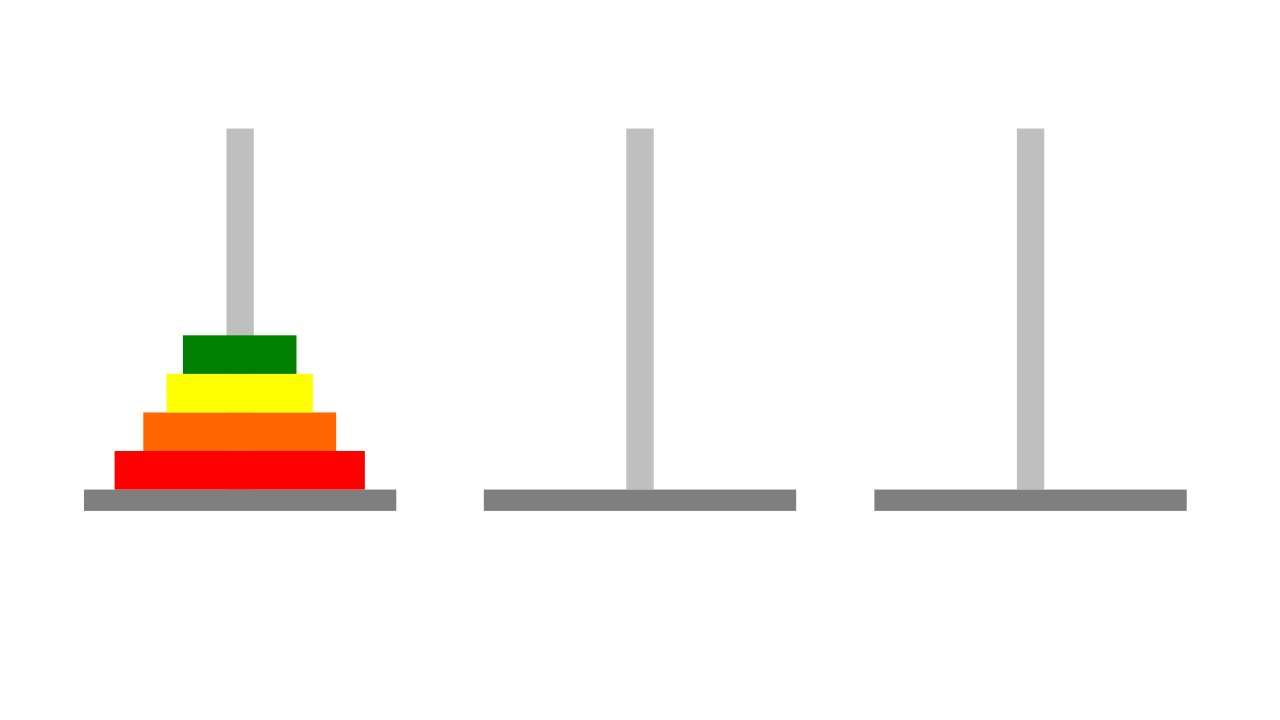
\includegraphics[scale=0.10]{torre.jpg}
				\end{minipage}
				
			\end{block}
		\end{frame}
	
	
\section{Ecuaciones de recurrencia}
\begin{frame}
	\frametitle{Ecuación de recurrencia de segundo orden}
	\begin{block}{Definición}
	$S_{n+2} = aS_{n+1} + bS_{n} + c, \;\; \forall\; n \; \textit{en el dominio de} \; S$
		 
	\end{block}
	\begin{block}{Teorema }
	\begin{itemize}
	    \item $S_n = A(r_1)^n + B(r_2)^n$ si $r_1 \neq r_2$, \;\;\;\;\;\;\;\;\;\;\;\;\;\;\;\;\;\; //Si $\Delta \neq 0$
	    \item $S_n = A(r)^n + Bn(r)^n$ si $r_1 = r_2 = r$, \;\;\;\;\;\;\;\;\;\;\; //Si $\Delta = 0$
	\end{itemize}
	\end{block}
\end{frame}

\begin{frame}
			\frametitle{Aplicación}
		\begin{block}{Modelo de la cunicultura\\
		$F_n = F_{n-1} + F_{n-2}$;  la ecuación de Fibonacci.}
				\begin{minipage}{7cm}
			Fibonacci partía de ciertas hipótesis, a saber:
\begin{itemize}
    \item Los conejos viven eternamente.
    \item Cada mes, un par de adultos de distinto sexo da lugar a un nuevo par de conejos de distinto sexo.
    \item Cada conejo se hace adulto a los dos meses de vida, momento en el que comienza a tener descendencia.
\end{itemize}		
				\end{minipage}\hspace{0.3cm}
				\begin{minipage}{4cm}
				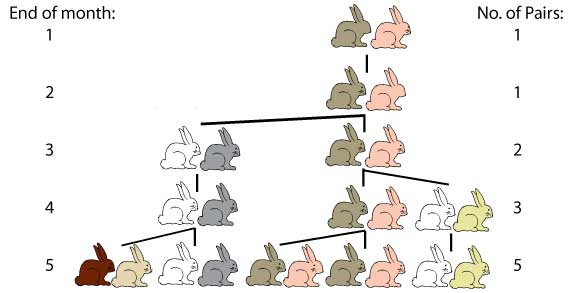
\includegraphics[scale=0.22]{conejos.jpg}
				\end{minipage}
				
			\end{block}
		\end{frame}

\end{document}